% This is lnicst.tex the demonstration file of the LaTeX macro package for
% Lecture Notes of the Institute for Computer Sciences, Social-Informatics 
% and Telecommunications Engineering series from Springer-Verlag.
% It serves as a template for authors as well.
% version 1.0 for LaTeX2e
%
\documentclass[lnicst]{svmultln}
%
\usepackage{graphicx} % includegraphics
\usepackage{makeidx}  % allows for indexgeneration
\usepackage{url} %for url citing
% \makeindex          % be prepared for an author index
%
\begin{document}
%
\mainmatter              % start of the contribution
%
\title{Obfuscation with Turing Machine}
%
\titlerunning{Turing Machine Obfuscation}  % abbreviated title (for running head)
%                                     also used for the TOC unless
%                                     \toctitle is used
%
\author{Yan Wang\inst{1} \and Dinghao Wu,\inst{2}
Shuai Wang \and Pei Wang}
%
\authorrunning{Ivar Ekeland et al.}   % abbreviated author list (for running head)
%
%%%% list of authors for the TOC (use if author list has to be modified)
\tocauthor{Ivar Ekeland, Roger Temam, Jeffrey Dean, David Grove,
Craig Chambers, Kim B. Bruce, Elisa Bertino}
%
\institute{Pennsylvania State University, State College,PA 16801, USA,\\
\email{ybw5084@ist.psu.edu},\\ WWW home page:
\texttt{http://users/\homedir iekeland/web/welcome.html}
% \and
% Universit\'{e} de Paris-Sud,
% Laboratoire d'Analyse Num\'{e}rique, B\^{a}timent 425,\\
% F-91405 Orsay Cedex, France}
}
\maketitle              
% typeset the title of the contribution
% \index{Ekeland, Ivar} % entries for the author index
% \index{Temam, Roger}  % of the whole volume
% \index{Dean, Jeffrey}

\begin{abstract}        % give a summary of your paper
Software security is a fundamental research domain in this threat emerging technology world. Leveraging system vulnerbilities is one of the common ways to hack into 
computer system. Hackers have to understand the program control flow in order to figure out the hacking logic and technique. In this way, consealing important branch trigger condition logics are crucial for protecting softwares from being hacked. In this paper we propose a novel control flow obfuscation method with Turing machine. By entwining the original software programs with Turing machine executio, software control flow graphs could be significantly obfuscated which means it is much more harder or even impossible for hackers to embed malicious execution codes into Turing machine obfuscated programs.We implemented a obfuscation tool to gernerate obfuscated binaries using LLVM. Evaluation results demonstrate that software programs become much more complicated after Turing maching obfuscation. At current stage, we only obfuscated the interger operand instructions which are vital to the whole program.
%                         please supply keywords within your abstract
\keywords {software security,control flow obfuscation, Turing machine,LLVM}
\end{abstract}
%
\section{Introduction}
%
Obfuscation derives from intellectual property protection. Internet brings us unprecedent convience and threat of idea plagiarism and copyright infringement at the same time.  Consealing the algorithm of a software means a lot for the society especially for high-tech industry. Reverse engineering is often used by to recover source code from binaries to analyze software vulnerbilities or to steal software ideas or algorithms. Obfuscation is a technique to block or harden the process of reverse engineering.

Recently, Software security has become a bigger and bigger concern in research community because of infamous ransomware attack and severe vulnerbiliy such as the recent ``Wanncry'' insidence and the openssl heartbleeding bug.This incidences challenge the computer world greatly. Hackers endevors to figure out vulnerbilities inside a software program. Knowing the software architecture and program logic like control flow graph is an indispensible prerequisite for hackers to analyze the original codes. With the help of some monitoring techniques hackers could even iterate all possible paths to try to restore all important branch information along the execution paths.\textit{Concolic testing} is an example which expoits symbolic execution given a certain input while it keeps changing input data until the code coverage proceed a threshhold\cite{Sen} as shown in Figure 1. It has been proved to work in restoring the branch information in the original source codes. Hence, a lot of research focus on preventing bad guys from figuring out the essential logic. Consealing important ``crossroad'' in a source program. Control flow obfuscation is one of these techniques. Control flow obfuscation aims at hiding conditional transfers and complicating the execution path within a source program. Through replacing or insering extra contrlo flow graph edges, the original software logic become harder or even impossible to trace. Previous research\cite{Ma} have prove the effectiveness of contral flow obfuscation.

\begin{figure}
  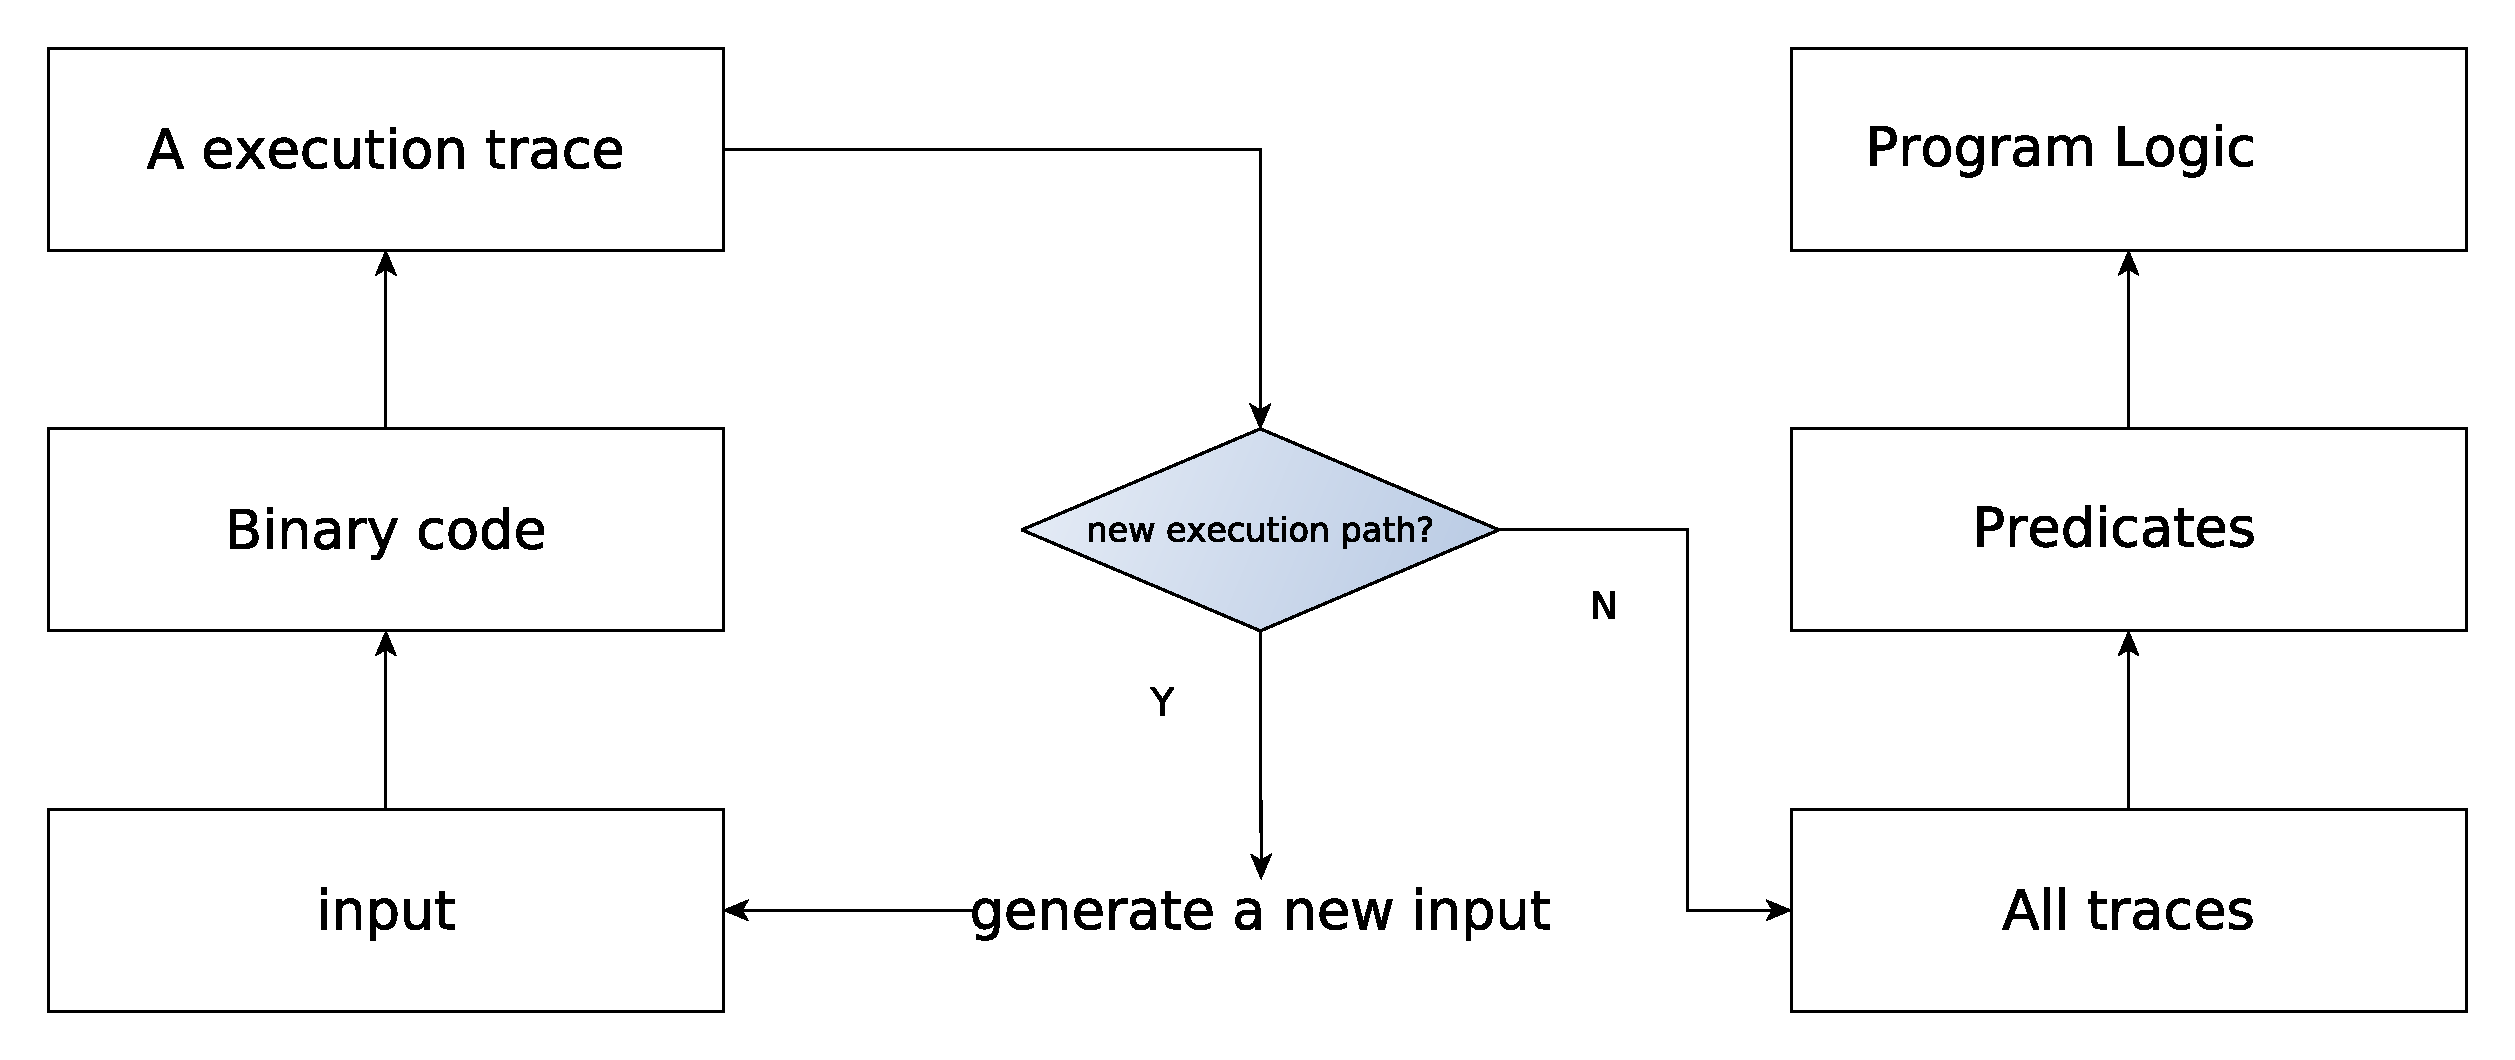
\includegraphics[width=0.9\linewidth]{reverse_engineering.eps}
  \caption{Reverse engineering with concolic testing}
  \label{Figure 1}
\end{figure}

In this paper,we propose a novel control flow obfuscation method with Turing machine embedded in the original program source codes. Turing machine is the essence of computaion so it could calculate accurately all kinds of computer operation. In this way, important branch conditions in original source code could be replaced by a Turing machine execution which yields the very identical conditional value. Besides, a Turing machine behaves like a state machine so it contains a lot of branch condition checks in Turing machine transition table. In this whole process, sensitive branch information could be successfully hided in Turing machine call graphs. In the mean time, Turing machine execution greatly introduce computational complexity to the target program so it is almost impossible to read the obfuscated programs to do reverse engineering. 

Currently, we are more interested in integer operation condition instructions. Utilizing LLVM, we could turn original program source codes into intermediate representation(IR).Turing machine obfuscator take over from IR and select interested instruction candidates which would be redirected to semantic equivalent Turing machine execution. After all paths finished in the Turing machine ``blackbox'', the original call graph resumes from the the obfuscator interrupt and the whole program control flow graph is greatly expanded and complicated. Since LLVM is the implementation foundation, currently our proposed obfuscator could only be applied to C/C++ source programs. Inspired by previous previous works\cite{Collberg},we evaluate our obfuscator from four demensions which are potency,resilence, cost and stealth respectively. Results indicates that Turing machin obfuscator could effectively obfuscate target source codes with acceptable cost overhead.

This paper is organized as follows. Section 2 discusses related works on obfuscation, especially control flow obfuscation. Section 3 illustrate the idea and archetecture of Turing machine obfuscator. Obfuscator implementation is discussed in section 4. Section 5 discusses the evaluation result of our proposed obfuscator. Finally, we conclude thsi paper in section 6.


%
\section{Related Works}
%
Generally speaking, reverse engineering is devided into static analysis such and dynamic analysis. To compete static reverse engineering, researchers usually focus on hardening disassembling and decompiling process. To compete the dynamic reverse engineering techniques such concolic testing, conditional transfer logic must be hidden from adversaries. Control flow obfuscation has been proved effective in previous works.

In \cite{Sharif}, the authors identified conditions that could trigger malware execution then using hash function to transform the values which could launch malware. Afterwards, correspondent conditional codes which would be ran with satisfied value were encryped with a key generated based on the instruction trigger value.
By this means the obfuscation analyzer could never get a chance to get the expected ``launching code'' consequently planted malware could never be executed. This technology works on certain fixed trigger value but not in senarios that trigger values are intervals such as \textgreater \   and  \textless. This limitation narrows the applicable conditions greatly since a large volume of branch conditions are comparsion operations. In addition, the encrytion and decryption process in this methodology also introduce inneglectable overhead.

In \cite{Popov}, the authors used signals(``traps'') to replace the control transfers unconditional instructions like ``jmp'' and ``call'' in order to confuse disassembly operation which is the first step of reverse engineering. Dummy control transfers and junk instructions were also inserted after signal replacements. This method seems to be effective in fooling disassemblers but it can't be applied in senarios that conditional instruction logic needs to be protected from being figured out.

In \cite{Zhi}, the authors endevors to conseal branch information leveraging a remote trusted third party environment. The idea seemed to work while it not only introduced a great network overhead, but also rely on trusted network accessiblity which can't be guranteed in reality. This drwaback means this idea can't be applied in common obfuscation cases.

In \cite{Ma}, the authors took advantage of neural network to replace appropriate conditional instructions in source programs in order to achieve the goal of consealing conditional instruction logic thus dynamic analysis like concolic testing could never dig useful branch information. Although the idea looks promising and the results indicates the effectiveness of this methodology to some degree, fundamentally we don't believe neural networks solution is suitable for such senarios. To the best of our knowledge,
neural networks works like a blackbox. It lacks the rigorous mathmatical proof to illustrate a correct result must be generated given a input. Neural networks not only introduced complexity but also unpredictability to the original source programs. Trained models may behave very differently if given initial parameters with only some nuances, which means that it is also very hard to train a accurate enough model to simulate the conditional instruction. In addition, we noticed that neural networks consume too much memory in the evaluation experiments.

%
\section{Turing machine obfuscation}
%
In a computer program, conditional transfer instruction compare two operands and direct the following running path based on the comparision result. In theory, Turing machine has been proved to be able to simulate any algorithm and generate a corresponding correct answer. If a problem could be solved mathmatically, it could definitely be solved by a Turing Machine. Taking advantage of Turing machine's powerful computational ability and mathematical correctness, we introduce Turing machine to the control flow obfuscation process. Through Turing machine computaion, the identical comparision result could be produced to guide further execution direction and the conditional logic is protected from being discovered. The intuitive methodology of Turing machine conditional branch transformation is shown in Figure 2.
\begin{figure}
 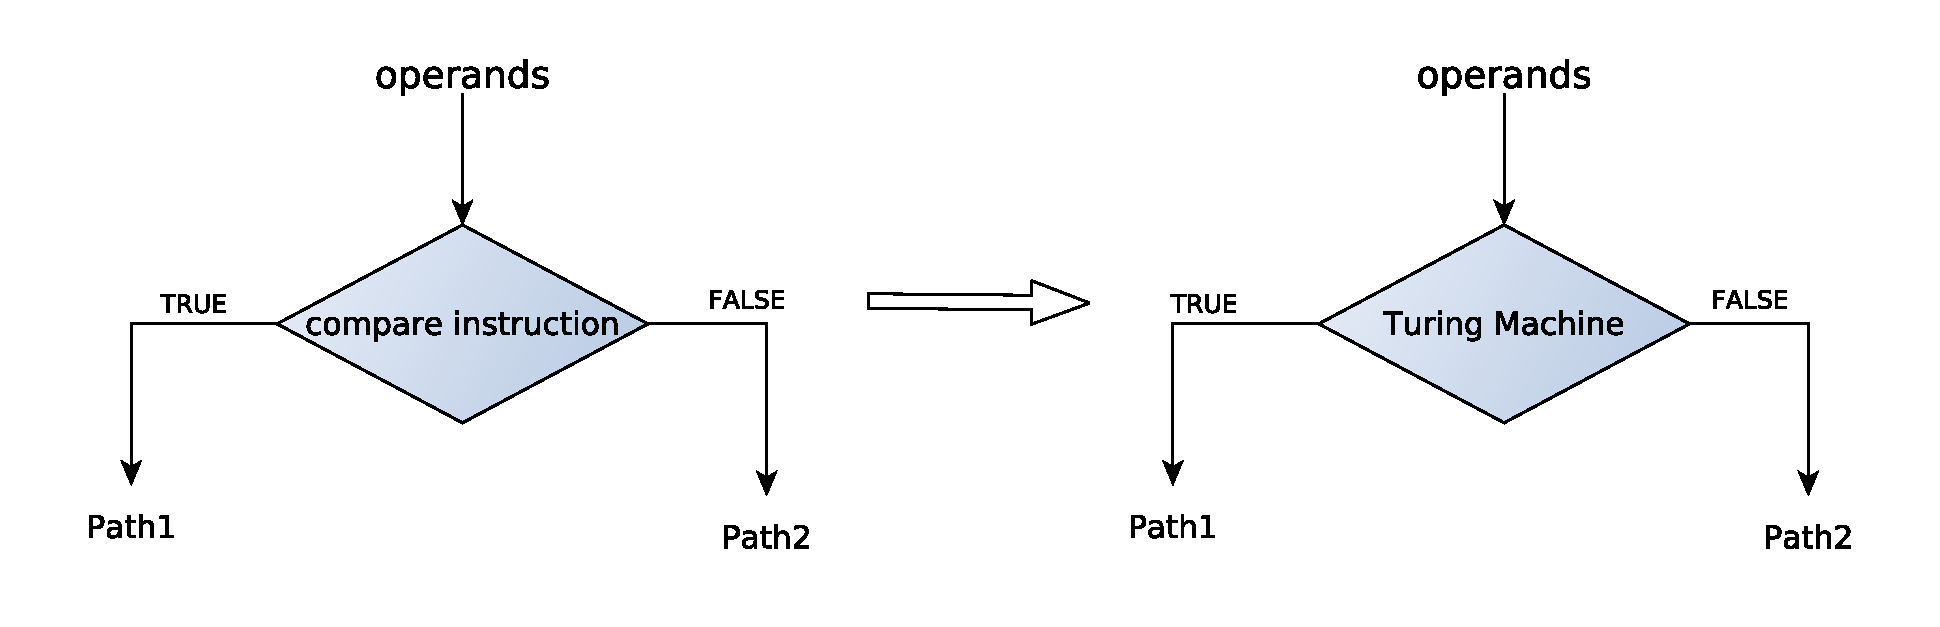
\includegraphics[width=\linewidth]{figure2.eps}
 \caption{Turing Machine Obfuscation Overview}
 \label{Figure 2}
\end{figure}
\subsection{Turing Machine}

\subsection{Universal Turing machine}

\section{Implementation}

\section{Evaluation}
Inspired by previous work\cite{Collberg}, we evaluated our obfuscation method based on four metrics which are \textit{potency}, \textit{resilience}, \textit{stealth} and \textit{cost} respectively. Potency indicates the complexity of a certain obfuscated program. It shows how complex or how unreadable obfuscated codes are. To measure how well an obfuscated program could withstand automatic deobfuscation techniques, metric resilience is introduced. Besides automated deobfuscators, a lot of reverse engineering works are conducted by hackers, obfuscated program should not be too different from the original one or it would be easy for experienced hackers to discern it. Stealth is used to measure to how well a obfuscated program resembles the original one. Cost is natually used the measure running overhead of a obfuscated program. Obfuscation would inevitably induce more overhead while it should be constricted to an acceptable level.

We choose two popular open source programs as target programs to verify effectiveness of our Turing machien obfuscator: compress tool bzip2\cite{bzip2} and regular expression engine slre\cite{slre}. In Turing machine obfuscator, we select integer conditional transfer instruction as replacement canditates. Obfuscation level is a index which indicates the ratio between obfuscated instructions and all instruction candidates. In our experiments, we arbitrarily set it to 50\% which means half of all conditional transfer candidates are randomly chosen and obfuscated.
\subsection{Potency}
%
Control flow graph(CFG) and call  graph provide useful information about the general structure of a program so they are the traditional foundation for static software analysis. With the help of IDA Pro\cite{ida} which is a well known commercial disassember and debuuger, CFG and call graph are generated from original and obfuscated binaries. Through analyzing both graphs, basic block number, call graph edge number and control graph edge number could be extracted. These static metrics are used to indicate complexity of a target program in \cite{Chen}. Experiment results are shown in table 1. Comparing the metrics of source program and corresponding Turing machine obfuscated program, we found program complexity is strenthened in terms of every metric.


\begin{center}
 \begin{tabular}{|c | c | c | c|} 
 \hline 
 Program & \# of CFG Edges & \# of Basic Blocks & \# of Function \\
 \hline
bzip2 & 4283 & 2837 & 78 \\ 
 \hline
obfuscated bzip2 & 4195 & 2828 & 134 \\
 \hline
regexp & 906 & 619 & 25 \\ 
 \hline
obfuscated regexp & 1122 & 773 & 43 \\
 \hline
\end{tabular}
\end{center}

Besides the traditional static evaluation, we refer to \cite{McCabe} and \cite{Woodward} to further quantify Turing machine obfuscated prgrams. Cyclomatic number and knot number were introduced in these works. Cyclomatic metric is defined by as \[ Cyclomatic = E - N + 2 \] where E and N represent the number of edge and node in a CFG respectively. Knot number means the quantity of edge crossings in the CFG. These two metris intuitively weighs how complicated a program is in terms of logic diverison number. Results in Table 2 show that both knot number and cyclomatic number increse after obfuscation. Potency of Turing machine obfuscator is proved.

\begin{center}
 \begin{tabular}{|c | c | c |} 
 \hline 
 Program & \# of Cylcomatic & \# of Knot \\
 \hline
bzip2 & 1448 & 11982  \\ 
 \hline
obfuscated bzip2 & 1369 & 5682  \\
 \hline
regexp & 289 & 478 \\ 
 \hline
obfuscated regexp & 351 & 1068 \\
 \hline
\end{tabular}
\end{center}

We pick 50\% as the obfuscation level to demonstrate the performance of Turing machine obfuscator while we also conducted experiments with other obfuscation level as \%30,\%80 and \%100. Figue 3 demostrated that with more control transfer instruction candidates transformed to Turing machine execution, binary call graph edges increases which indicates obfuscated binary become more and more complicated. 
\begin{figure}
  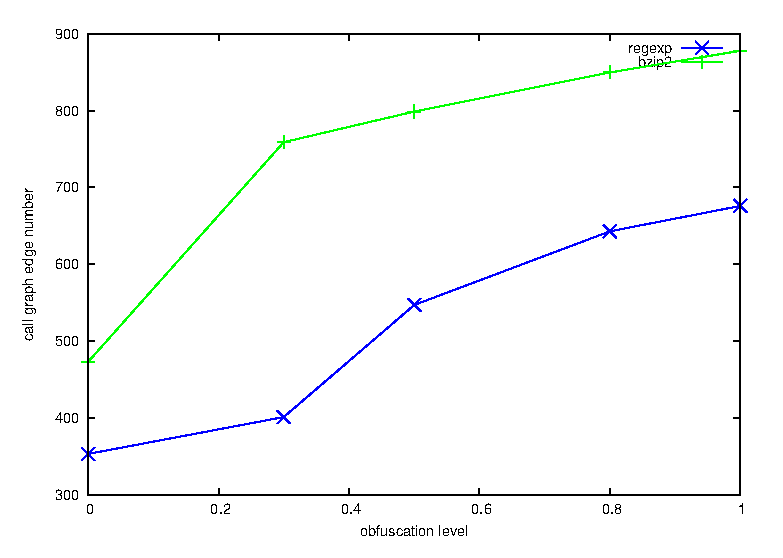
\includegraphics[width=0.9\linewidth]{cg.eps}
  \caption{Call graph Edge Number versus obfuscatio level}
  \label{Figure 3}
\end{figure}
\subsection{Stealth}
As mentioned in previous section, software obfuscation technique should not only combat automated deobfuscation tools, but also manual deobfuscation methods. In the evaluation of stealth, authors of \cite{Trans} calculated the statistics of instruction distribution of both regular and obfuscated programs to draw a comparison. If instruction distribution statistics of a obfuscated program is distinct from normal programs(e.g call instruction proportion is abnormally high), it would be easy for reverse engineer to discern the program has been instrumented. We employed this same metric to evaluate our Turing obfuscator. Obfuscation level for stealth evaluation is set to 50\%.
\begin{figure}
  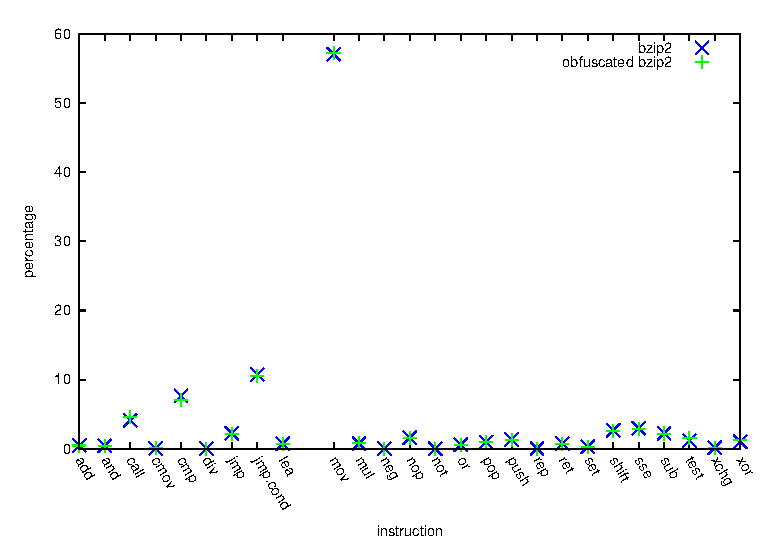
\includegraphics[width=0.9\linewidth]{st_bzip2.eps}
  \caption{bzip2 instruction distribution comparison}
  \label{Figure 4}
\end{figure}

\begin{figure}
  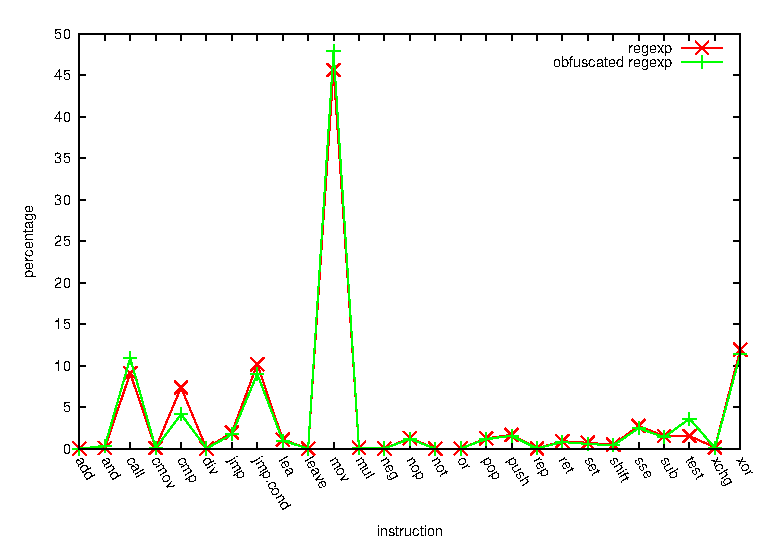
\includegraphics[width=0.9\linewidth]{st_regexp.eps}
  \caption{regexp instruction distribution comparison}
  \label{Figure 5}
\end{figure}
 We classfied binary instructions into 27 different classes. Figure 4 and Figure 5 present the instruction distribution of the original and obufuscated version of target programs(bzip2 and regexp). Experiment results indicates that the instruction distribution after obfuscation is close to the origin distribution. Given the fact that obfuscated binaries contains extra instructions of Turing machine obfuscator, obfuscated slre changed more than obfuscated bzip2 since the former binary contains 1391 lines of code and the later binary contains only 1391 lines of code. After all, Turing machine obfuscator is proved to obfuscate source binaries with good stealth performance because of small instruction distribution variation.

\section{Cost}

%
% ---- Bibliography ----
%
\begin{thebibliography}{5}

\bibitem{Sen} Sen, Koushik, Darko Marinov, and Gul Agha. "CUTE: a concolic unit testing engine for C." ACM SIGSOFT Software Engineering Notes. Vol. 30. No. 5. ACM, 2005.

\bibitem{Ma} Ma, Haoyu, et al. "Control flow obfuscation using neural network to fight concolic testing." International Conference on Security and Privacy in Communication Systems. Springer International Publishing, 2014.

\bibitem{Trans} Wang, Pei, et al. "Translingual obfuscation." Security and Privacy (EuroS\&P), 2016 IEEE European Symposium on. IEEE, 2016.

\bibitem{Collberg} Collberg, Christian, Clark Thomborson, and Douglas Low. "Manufacturing cheap, resilient, and stealthy opaque constructs." Proceedings of the 25th ACM SIGPLAN-SIGACT symposium on Principles of programming languages. ACM, 1998.

\bibitem{Sharif} Sharif, Monirul I., et al. "Impeding Malware Analysis Using Conditional Code Obfuscation." NDSS. 2008.

\bibitem{Popov} Popov, Igor V., Saumya K. Debray, and Gregory R. Andrews. "Binary Obfuscation Using Signals." Usenix Security. 2007.

\bibitem{Zhi} Wang, Zhi, et al. "Branch obfuscation using code mobility and signal." Computer Software and Applications Conference Workshops (COMPSACW), 2012 IEEE 36th Annual. IEEE, 2012.

\bibitem{bzip2} \url{http://www.bzip.org/}

\bibitem{slre} \url{https://github.com/cesanta/slre}

\bibitem{Chen} Chen, Haibo, et al. "Control flow obfuscation with information flow tracking." Proceedings of the 42nd Annual IEEE/ACM International Symposium on Microarchitecture. ACM, 2009.

\bibitem{ida} \url{https://www.hex-rays.com/products/ida/}

\bibitem{McCabe} McCabe, Thomas J. "A complexity measure." IEEE Transactions on software Engineering 4 (1976): 308-320.

\bibitem{Woodward} Woodward, Martin R., Michael A. Hennell, and David Hedley. "A measure of control flow complexity in program text." IEEE Transactions on Software Engineering 1 (1979): 45-50.
%%


\end{thebibliography}
%
\end{document}
